\section{Introduction}
Electric-vehicle (EV) adoption in India is strikingly uneven. Across the four states studied here, the EV share of new registrations in 2025 ranged from about 8\% in Maharashtra and Tamil Nadu to 14.9\% in Delhi, although all four operate under the same national incentive framework. For manufacturers, charging operators and state agencies this is a business problem: capital for dealerships, chargers and subsidies is finite, and a wrong regional bet is costly to reverse. Operational public stations rose from 6{,}586 nationally in March 2023 \cite{pib23} to 12{,}146 in February 2024 \cite{pib24}; a December 2025 reply reports 29{,}151 installed over five years \cite{pib25}.

Few studies tell a regional decision-maker \emph{both} what is likely to happen \emph{and} which regional factors are associated with it, while being honest about what a small public data set supports. We build a two-layer pipeline---an explanatory layer (tree models with SHAP) and a forecasting layer (statistical, ML and ensemble models under three out-of-sample tests)---on a state--month panel from Vahan registrations \cite{vahan} and five other public sources.

\subsection{Scope and Objectives}
The project explains and forecasts state-level EV adoption with an interpretable, multi-source pipeline. Its objectives are to (i) establish the relevance of regional EV disparities; (ii) show originality by coupling driver explanation with out-of-sample forecasting on an \emph{adoption-rate} target; (iii) achieve robust, honestly validated results; and (iv) ensure reproducibility. Four research questions guide the work: \textbf{RQ1} how has EV adoption evolved across the states; \textbf{RQ2} which economic, environmental and infrastructure variables are most associated with it; \textbf{RQ3} do models with exogenous drivers forecast better than classical baselines; \textbf{RQ4} can explainable ML give region-specific insights.

\section{Related Work}
\emph{Determinants.} Cross-country regressions find charging infrastructure the factor most related to EV market share \cite{sierzchula}; structural work on US metropolitan areas shows two-sided feedback between sales and chargers \cite{li}, warning that driver--adoption associations may run in both directions. \emph{Forecasting in India.} Vahan-based studies compare regression models on category sales \cite{devarasan}, forecast monthly two-wheeler registrations with SVM, forest and boosted trees \cite{rohit}, or project electric two-wheeler diffusion to 2035 with a Bass model \cite{radhakrishnan}; outside India, deep hybrids forecast model-level US sales \cite{afandizadeh}. \emph{Methods.} Tree ensembles \cite{chen,ke,breiman} are strong on medium-sized tabular data \cite{grinsztajn}; SHAP \cite{lundberg} attributes predictions to features; simple statistical methods are often competitive on short series \cite{makridakis} and combining forecasts usually helps \cite{bates}. We combine these threads on an adoption-rate target and report where the data cannot support a conclusion.

\section{Methodology}
\subsection{Data and provenance}
The panel has four states $\times$ 58 months (January 2022--October 2026); registrations are used through September 2026 (October is a partial month, dropped), i.e.\ 228 state-months with 2.60 million EV registrations out of 32.3 million (8.0\%). The target is $y_{s,t}=100\times\text{EV}_{s,t}/\text{total}_{s,t}$. Table~\ref{tab:data} lists sources and specifications. Air quality comes from one metro station per state and weather from the mean of four representative cities per state (proxies). Sep--Oct 2026 air-quality, weather and fuel values were identical across states (placeholders) and are treated as missing, so same-month explanatory models stop at August 2026. Seventeen same-month columns (EV count, totals, fuel and category splits) are excluded as predictors because they contain or define the target. After VIF pruning (PM$_{10}$, PM$_{2.5}$, diesel price dropped) eight drivers remain: AQI, NO$_2$, SO$_2$, petrol price, charging stations, per-capita GSDP, temperature and rainfall.

\begin{table*}[!t]
\caption{Data Sources and Alignment (full specification, corrections log and attestation items in the repository)}\label{tab:data}
\centering\footnotesize
\begin{tabular}{p{2.9cm}p{7.0cm}p{2.0cm}p{4.9cm}}
\toprule
\textbf{Variable} & \textbf{Source and specification} & \textbf{Granularity} & \textbf{Alignment / assumed release}\\
\midrule
EV and total registrations & MoRTH Vahan dashboard \cite{vahan} (downloaded Oct. 9, 2026); state, month-wise, fuel and vehicle-category views; EV = electric fuel & State--month & Target; not a predictor\\
AQI, PM, NO$_2$, SO$_2$ & CPCB CAAQMS \cite{cpcb}; daily averages, one station per state (Delhi, Mumbai--Bandra, Chennai--Alandur, Kolkata--Victoria) & Daily $\to$ month & Visible 1 month later\\
Temperature, rainfall & NASA POWER point API \cite{nasa}: T2M, PRECTOTCORR, mean of four cities per state & Monthly & Visible 1 month later\\
Petrol, diesel price & PPAC metro retail prices \cite{ppac} (Delhi, Mumbai, Chennai, Kolkata) & Daily $\to$ month & Visible 1 month later\\
Public charging stations & PIB/Parliament snapshots: Mar-2023 and Feb-2024 (\emph{operational}) \cite{pib23,pib24}, Dec-2025 (\emph{installed in last five years}) \cite{pib25}, Aug-2026 \cite{sansad,ians26} & 4 snapshots per state & Release = label + 1 month; never back-filled (first snapshot fills Jan-2022--Feb-2023, flagged)\\
GSDP per capita, current prices & MoSPI and state economic surveys \cite{mospi}, gross per capita by financial year: 2022--23 actual, 2023--24 revised, 2024--25 and 2025--26 advance, 2026--27 projected (budget-derived) & Financial year & Visible 24 months after the FY starts \cite{rbi}; the projected value never enters a forecast\\
\bottomrule
\end{tabular}
\end{table*}

\textit{Vintage alignment.} A forecast made at origin $o$ may use only values published by $o$. Monthly covariates are lagged one month, each charging snapshot becomes visible at an explicit assumed release month, and GSDP 24 months after its financial year starts; no value is back-filled to earlier months. These release dates are assumptions. The charging series is not like-for-like (two snapshots count operational stations, one five-year installations; several Aug-2026 values are approximate); two entries of the first compilation were corrected against the PIB annexures (Maharashtra Feb-2024: 3{,}079, not 3{,}728; an unsourced ``end-2022'' row replaced by the official March-2023 row).

\textit{West Bengal.} West Bengal's share jumped to 23.6\% in November 2025 and decayed over three months (flagged November 2025--February 2026). In those months excess EVs were 1.01 times excess three-wheelers (correlation 0.98), while no other state shows such a jump. This is \emph{evidence consistent with} an e-rickshaw registration backlog following a state mandate (trade-press report \cite{emobility}); it is not an official verification. The ``backlog-removed'' series, which subtracts the three-wheeler excess over its pre-episode median, is an assumption-based sensitivity treatment, not corrected ground truth. Headline accuracy metrics exclude the flagged months.

\subsection{Models and Evaluation Design}
\textit{Explanatory layer (same-month).} Ridge, random forest, XGBoost and LightGBM regress the adoption rate on the drivers (hyper-parameters tuned on 2022--24 expanding folds only). SHAP \cite{lundberg} is cross-checked by fixed-effects regressions of $\log y$ with state and month effects (A) and an added trend (B), HAC errors \cite{neweywest}. A driver is \emph{robust} only if SHAP and both specifications agree in sign and are significant at 10\%.

\textit{Forecasting layer.} For horizons $h=1,\dots,6$, one global model per horizon predicts $\log(y_{t}/b_o)$, $b_o$ being the mean of the last three observed months. Feature sets: F0 history only (level, momentum, year-on-year, seasonal terms), F1 adds lagged air quality, petrol price and weather, F2 adds charging and GSDP, all vintage-aligned. Models: naive, 3-month average, seasonal naive, damped ETS \cite{hyndman}, per-state SARIMA \cite{box}, a pooled-seasonal damped-trend model, and Ridge, LightGBM and XGBoost on F0--F2, tuned by randomised search on pre-origin data only. \emph{Model status matters:} the \textbf{pre-declared primary} model is the equal-weight ensemble of the three best F0 models on the 2024 validation window (SARIMA, ETS, XGBoost-F0), a rule fixed before the 2025--26 results were read. The equal-weight pool of seven F0 models and a SARIMA that averages four specifications were added \emph{after} test results were seen and are \textbf{exploratory}; we show them but do not treat their ranking as confirmatory. LSTM and Prophet were not run ($\approx$57 monthly points per state are too few).

\textit{Three tests, never pooled.} \textbf{E1} rolling origin: every target month January 2025--September 2026 forecast from origins 1--6 months earlier ($21$ months $\times$ 4 states $\times$ 6 horizons $=504$ forecasts, 480 excluding flagged West Bengal months). \textbf{E2} fixed origin: everything (tuning, specifications, intervals) estimated on data to March 2026, then April--September 2026 forecast and compared with actuals ($6\times4=24$ forecasts, one origin). \textbf{E3} frozen forecasts, scored when actuals arrive. Metrics are MAE, RMSE, sMAPE and R$^2$ in pp of adoption rate and skill against the last-value naive forecast; differences use a paired block bootstrap over target months (4{,}000 resamples, 90\% interval); 80\% intervals use empirical log-error quantiles realised before each origin.

\section{Results}
\subsection{Adoption Patterns (RQ1)}
Adoption rose in every state while the ranking stayed Delhi, Maharashtra, Tamil Nadu, West Bengal until 2026 (Fig.~\ref{fig:eda}a). Annual volume-weighted shares moved from 10.2\% (2022) to 14.9\% (2025) in Delhi, 5.7\% to 8.6\% in Maharashtra (flat in 2024--25), 3.9\% to 8.2\% in Tamil Nadu and 1.2\% to 8.0\% in West Bengal (including the flagged months); January--August 2026 shows a further step up in Maharashtra (11.2\%) and Tamil Nadu (10.6\%). The pooled STL index peaks in March (1.25, fiscal year-end) and December (1.23) and bottoms in January (0.82) (Fig.~\ref{fig:eda}b).

\begin{figure*}[!t]
\centering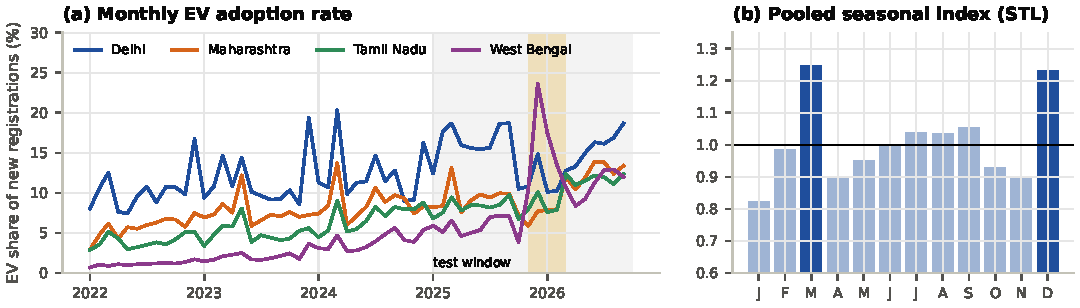
\includegraphics[width=\textwidth]{figs/fig1_eda.pdf}
\caption{(a) Monthly EV adoption rate by state; shading marks the flagged West Bengal months (yellow) and the 2025--26 test window (grey). (b) Pooled seasonal index from STL decomposition \cite{cleveland}.}\label{fig:eda}
\end{figure*}

\subsection{Drivers of Adoption (RQ2, RQ4)}
\textit{Predictive value.} On the 2025--26 hold-out the same-month driver models reach R$^2$ of only 0.13--0.20 (Ridge 0.20, LightGBM 0.19) against 0.07 for ``the state's 2024 mean''; leave-one-state-out R$^2$ ranges from 0.01 to 0.47. They are tools for explanation, not prediction.

\textit{Driver ranking.} Charging stations top the SHAP ranking (mean $|\phi|$ = 2.17 pp), followed by GSDP per capita (0.66), petrol price (0.36), SO$_2$ (0.21) and NO$_2$ (0.19); the other drivers are below 0.10 (Fig.~\ref{fig:shap}a). The ranking is stable when a state is removed (Spearman 0.96--0.99). By state (RQ4, Fig.~\ref{fig:shap}b), charging stock adds 2.4 pp in Delhi and 0.9 pp in Maharashtra but subtracts 1.1 pp in Tamil Nadu and 2.0 pp in West Bengal; income adds 1.0 pp in Delhi and subtracts 1.0 pp in West Bengal; air quality and weather contribute under 0.6 pp everywhere.

\begin{figure*}[!t]
\centering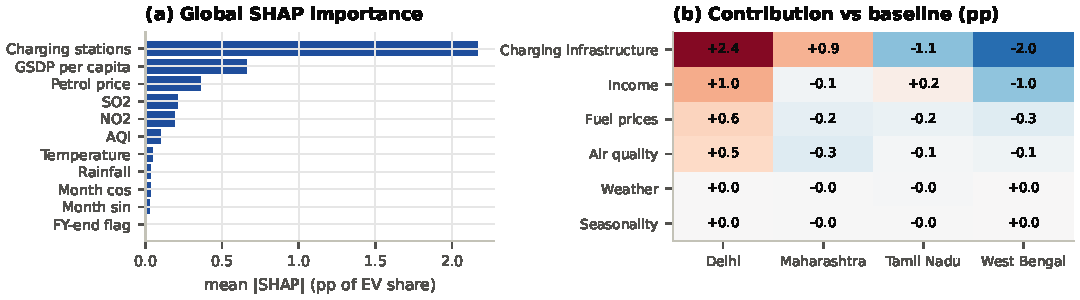
\includegraphics[width=\textwidth]{figs/fig2_shap.pdf}
\caption{(a) Mean absolute SHAP value by feature (random forest, all months through August 2026). (b) Average contribution of each driver group to each state's predicted EV share relative to the 8.1\% baseline (pp).}\label{fig:shap}
\end{figure*}

\textit{How far can this be trusted?} Table~\ref{tab:drivers} triangulates the evidence. Between-state differences account for 55\% of the SHAP variance of charging stations, 70\% for GSDP and 76\% for petrol price, so these ``drivers'' largely identify \emph{which state} a row belongs to; charging and GSDP are step series. In the fixed-effects regressions the GSDP coefficient flips from $+114\%$ to $-67\%$ per SD once a trend is added, the charging coefficient changes sign, and none of the eight drivers is significant at 10\% in both specifications with a matching SHAP sign: \textbf{no driver is robust}. We therefore report associations only. What-if runs on the explanatory models agreed on the sign in only 33\% of scenario cells and are not interpreted as elasticities.

\begin{table}[!t]
\caption{Triangulation of Driver Evidence (n=224, through Aug-2026)}\label{tab:drivers}
\centering\footnotesize
\setlength{\tabcolsep}{3pt}
\begin{tabular}{lcccccc}
\toprule
\textbf{Driver} & \textbf{$|\phi|$} & \textbf{SHAP} & \multicolumn{2}{c}{\textbf{FE effect, \%/SD}} & \textbf{Verdict}\\
 & \textbf{(pp)} & \textbf{sign} & \textbf{A} & \textbf{B} & \\
\midrule
Charging stations & 2.17 & $+$ & $+$2.0 & $-$8.1* & fragile\\
GSDP per capita & 0.66 & $+$ & $+$114* & $-$67* & fragile\\
Petrol price & 0.36 & $-$ & $+$5.1 & $+$9.6* & fragile\\
SO$_2$ & 0.21 & $+$ & $-$5.1$^{\dagger}$ & $-$2.1 & fragile\\
NO$_2$ & 0.19 & $+$ & $-$1.8 & $-$4.5 & fragile\\
AQI & 0.10 & $+$ & $-$2.1 & $-$2.9 & fragile\\
Temperature & 0.04 & $-$ & $-$1.6 & $-$8.4 & fragile\\
Rainfall & 0.03 & $-$ & $+$7.6* & $+$1.1 & fragile\\
\bottomrule
\multicolumn{6}{p{8.0cm}}{\scriptsize *p$<$0.05, $^{\dagger}$p$<$0.10 (HAC). A: state and month effects; B: A plus linear trend. Robust = same sign in SHAP, A and B and p$<$0.10 in both A and B.}\\
\end{tabular}
\end{table}

\subsection{Forecast Accuracy (RQ3)}
Table~\ref{tab:fc} reports every accuracy figure with its exact sample; rows from different tests must not be compared.

\begin{table*}[!t]
\caption{Forecast Accuracy by Test (MAE, RMSE in pp of EV share; skill = MAE reduction vs naive)}\label{tab:fc}
\centering\footnotesize
\begin{tabular}{p{4.6cm}p{4.0cm}ccccc}
\toprule
\textbf{Test and sample} & \textbf{Model (status)} & \textbf{MAE} & \textbf{RMSE} & \textbf{R$^2$} & \textbf{Skill} & \textbf{Forecasts}\\
\midrule
\multirow{5}{4.6cm}{E1 rolling origin, targets Jan-25--Sep-26 (21 months), $h$=1--6, state level, flagged WB excluded}
 & \textbf{Top-3 ensemble (pre-declared)} & \textbf{1.94} & 2.64 & 0.47 & 17.1\% & 480\\
 & SARIMA (per state) & 1.93 & 2.64 & 0.48 & 17.5\% & 480\\
 & Equal-weight F0 pool (exploratory) & 1.90 & 2.61 & 0.49 & 18.8\% & 480\\
 & SARIMA, 4 specs averaged (exploratory) & 1.84 & 2.61 & 0.49 & 21.4\% & 480\\
 & Naive (last value) & 2.34 & 3.25 & 0.21 & --- & 480\\
\midrule
E1 split: 2025 targets (12 months) & Top-3 / naive & 1.53 / 1.94 & 2.14 / 2.70 & 0.71 / 0.54 & 21.3\% & 276\\
E1 split: Jan--Sep 2026 targets (9 months) & Top-3 / naive & 2.51 / 2.89 & 3.20 / 3.87 & $-$0.52 / $-$1.21 & 13.2\% & 204\\
E1 sensitivity: flagged WB months included & Top-3 / naive & 2.23 / 2.68 & 3.26 / 3.94 & 0.30 / $-$0.02 & 16.9\% & 504\\
\midrule
\multirow{4}{4.6cm}{E2 fixed origin Mar-2026, targets Apr--Sep 2026 (6 months), $h$=1--6, state level}
 & \textbf{Top-3 ensemble (pre-declared)} & \textbf{2.41} & 2.73 & $-$0.34 & $-$41.5\% & 24\\
 & SARIMA (per state) & 1.96 & 2.42 & $-$0.05 & $-$15.6\% & 24\\
 & Equal-weight F0 pool (exploratory) & 2.58 & 2.97 & $-$0.59 & $-$52.0\% & 24\\
 & Naive (last value) & 1.70 & 2.19 & 0.14 & --- & 24\\
\midrule
E3 pooled four-state series, Jan-25--Sep-26, $h$=1--6 (not India) & SARIMA-avg4 (exploratory) / naive & 1.00 / 1.64 & 1.30 / 2.04 & 0.57 / $-$0.05 & 39.2\% & 102\\
\bottomrule
\end{tabular}
\end{table*}

\textit{Rolling origin (E1, RQ3).} The pre-declared top-3 ensemble reaches MAE 1.94 pp, 0.40 pp below the last-value naive benchmark (90\% interval $-0.64$ to $-0.18$), but its difference from per-state SARIMA is $+0.01$ pp (interval $-0.11$ to $+0.12$): the leading models are statistically tied. The exploratory pool and SARIMA-avg4 are slightly lower (1.90, 1.84), yet they were added after results were seen, so their rank is not evidence. Error grows with horizon (top-3: 1.48 pp at one month, 2.12 at six) and is hardest for Delhi (3.58) and easiest for Tamil Nadu (1.07). Accuracy fell in 2026 (2.51 vs 1.53 pp in 2025), when R$^2$ turned negative. Pooled R$^2$ is moderate (0.47; within-state $-0.11$). \textbf{Covariates hurt:} relative to F0, F2 raised MAE by 0.15 pp (Ridge), 0.07 (LightGBM) and 0.08 (XGBoost), significantly in all three, and F1 raised it by 0.09 (Ridge, significant), 0.04 and 0.07 (not significant): four of six comparisons are significantly worse, none better. The 80\% intervals covered 75\% of outcomes (88\% at one month, 60\% at six), so long-horizon intervals are too narrow.

\begin{figure*}[!t]
\centering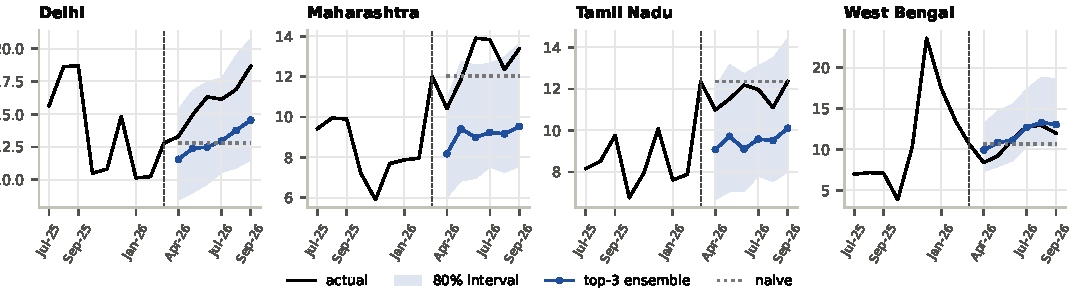
\includegraphics[width=\textwidth]{figs/fig3_backtest.pdf}
\caption{Fixed-origin backtest (E2): models trained to March 2026 (dashed line) forecast April--September 2026; the pre-declared top-3 ensemble with its 80\% interval, the naive forecast and the actual outcome (EV share, \%).}\label{fig:bt}
\end{figure*}

\textit{Fixed-origin backtest (E2).} Trained to March 2026 and scored on the six months that followed, the top-3 ensemble has MAE 2.41 pp against 1.70 for the naive forecast: \textbf{it does not beat the naive benchmark} (Fig.~\ref{fig:bt}; $-41.5\%$ skill; rank 4 of 12 models, with only the naive and per-state SARIMA below it). The reason is a 2026 level shift: Delhi, Maharashtra and Tamil Nadu were under-forecast by 3.1, 3.5 and 2.2 pp on average. March is a fiscal-year-end spike every year, so seasonal models forecast a fall-back that did not materialise, whereas the naive forecast carried the high March level forward. West Bengal was forecast well (0.81 pp). The 80\% interval nevertheless contained 22 of 24 outcomes because it is wide. A single origin gives only 24 forecasts, so this is a stress test, not a ranking: scoring the \emph{same} April--September 2026 targets over all rolling origins gives 2.42 pp for the top-3 ensemble against 2.85 for naive. Nothing was retuned after seeing this result. In the backtest, covariates did not help consistently either (F2$-$F0: $-0.05$, $-0.00$, $-0.13$ pp for Ridge, LightGBM, XGBoost; $n=24$), and treating the flagged West Bengal months as a backlog \emph{worsened} West Bengal's backtest error (3.84 vs 0.81 pp), a warning that the adjustment is an assumption.

\textit{Prospective check (E3).} The forecast frozen on 11 November 2026 (origin August) was scored on September 2026: MAE 0.97 pp over four state forecasts, all inside the 80\% intervals. With $n=4$ this is anecdotal; the refit forecast below is frozen for scoring.

\subsection{Outlook for October 2026--March 2027}
Refit on all data (September 2026 origin), the pre-declared ensemble projects the paths in Table~\ref{tab:outlook} and Fig.~\ref{fig:fc}. The other three states barely depend on the West Bengal treatment ($\le1.3$ pp). For West Bengal the two treatments bracket the plausible range: taken as reported, a seasonal model replays the winter spike (26\% in December 2026), which we regard as an artefact; with the assumed backlog removed the forecast is 8--11\%, yet this treatment did worse in the backtest. We therefore present West Bengal as a range and do not choose between the two. All paths reproduce the March fiscal-year-end spike (Delhi 19.1\%, 80\% interval 15.0--27.4\%; Maharashtra 15.6\%, 12.2--22.3\%). Given the backtest, these ranges should be read as planning scenarios that may under-state a continued 2026 level shift.

\begin{table}[!t]
\caption{Forecast EV Share (\%), Pre-Declared Top-3 Ensemble, Origin Sep-2026}\label{tab:outlook}
\centering\footnotesize
\setlength{\tabcolsep}{3.4pt}
\begin{tabular}{lccccc}
\toprule
\textbf{Month} & \textbf{Delhi} & \textbf{Maha.} & \textbf{T. Nadu} & \multicolumn{2}{c}{\textbf{West Bengal}}\\
 & & & & as rep. & backlog rem.\\
\midrule
Oct-26 & 14.1 & 10.5 & 9.9 & 9.1 & 8.9\\
Nov-26 & 13.3 & 8.5 & 10.4 & 14.2 & 8.0\\
Dec-26 & 18.2 & 9.9 & 12.7 & 26.1 & 11.0\\
Jan-27 & 14.4 & 9.9 & 9.8 & 20.4 & 10.1\\
Feb-27 & 16.2 & 10.9 & 10.9 & 18.4 & 10.6\\
Mar-27 & 19.1 & 15.6 & 15.4 & 18.8 & 17.9\\
\bottomrule
\end{tabular}
\end{table}

\begin{figure*}[!t]
\centering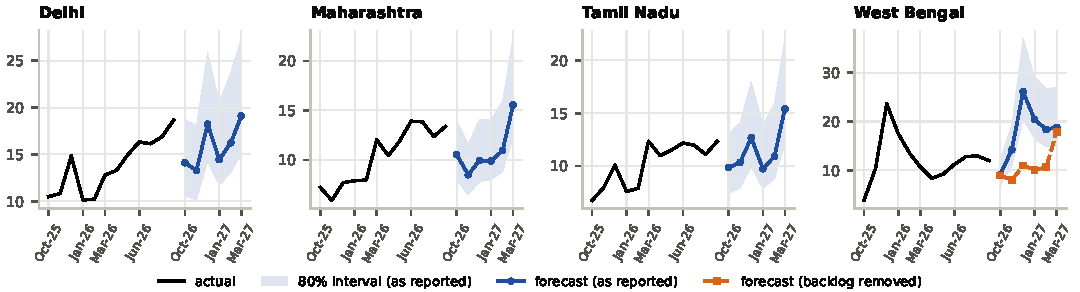
\includegraphics[width=\textwidth]{figs/fig4_forecast.pdf}
\caption{Forecast of EV adoption rate, October 2026--March 2027, with 80\% intervals (as-reported history); West Bengal also shows the backlog-removed treatment (EV share, \%).}\label{fig:fc}
\end{figure*}

\section{Discussion}\label{sec:disc}
\textit{Relevance (objective i, RQ1).} Disparities are large and persistent: 2025 shares range from 8\% to 15\%, and public chargers in August 2026 range from about 1{,}200 (West Bengal) to 6{,}985 (Maharashtra). Manufacturers can use the seasonal calendar and forecast ranges; operators should note that charging stock tops the SHAP ranking, in line with \cite{sierzchula}, but this data cannot show that adding chargers raises adoption (reverse causality is plausible \cite{li}).

\textit{Originality and honest validation (objectives ii, iii; RQ2--RQ4).} We model an adoption rate and couple explanation with forecasting under release-aligned covariates. The main finding is negative: once publication dates are respected, drivers add no forecast accuracy and none is robust. We separate the pre-declared model from exploratory ones and report the failed backtest. All objectives are met except the LSTM/Prophet benchmarks.

\textit{Limitations.} (i) Four states; covariates have effectively four cross-sectional points. (ii) Air quality is one station per state and weather a four-city average (Delhi's include Gurugram, Noida, Faridabad); GSDP is gross per capita from mixed state and national releases. (iii) Charging has four snapshots with a definition break, estimated Aug-2026 values for Delhi and West Bengal; GSDP beyond 2022--23 is revised, advance or projected. (iv) Release dates are assumptions. (v) SHAP and regressions give associations only. (vi) The West Bengal episode is consistent with, not officially verified as, a registration backlog. (vii) The backtest has 24 forecasts from one origin.

\textit{Recommendations.} (1) Plan with ranges, not points, and refresh monthly. (2) Build capacity plans around the seasonal index but stress-test for a level shift. (3) Before investing in chargers, assemble district-level, consistently defined counts and vehicle-class splits. (4) Obtain the official West Bengal registration notification. (5) Test local-trend state-space and panel models, pre-declared, in future work.

\section{Reproducibility}
Code, data, reference tables, the corrections log and an executed notebook are at \texttt{https://github.com/AravindGupta-Podduturi/ev-adoption-india}. After \texttt{pip install -r requirements.txt}, \texttt{python run\_all.py} regenerates every table and figure (about 3.5 minutes on two CPU cores in a clean run); seed 42; tuning uses pre-origin data only. Stage \texttt{11} writes the master results table behind every number here. % MANUAL: paste your GitHub URL

\subsection{AI Use Declaration}
Claude helped structure the workflow, find public sources and literature, write analysis code and draft this report from the team's outputs; Google Gemini helped draft the panel-building and NASA POWER scripts. The team reviews all AI-assisted text and code against the data; AI-generated content must stay under 20\% of the submission \emph{[team to confirm before submission]}. % MANUAL: confirm AI share <=20pct, delete bracket

\section{Conclusion}
A two-layer pipeline on a four-state panel shows that regional EV adoption is rising, strongly seasonal, and forecast reasonably by simple combinations of SARIMA, ETS and ML models over many origins (MAE 1.94 pp, 17\% below naive), but not in a stress test that began just before a 2026 level shift, where the naive forecast won. Charging stock tops the SHAP ranking, yet no driver is robust and covariates do not improve forecasts, so findings should guide data collection, not investment sizing. Future work should add districts and vehicle classes, verify the West Bengal registrations, and test a pre-declared local-trend model.

\section*{Acknowledgment}
The authors thank Instructor Suman Sanyal Sir for guidance and feedback throughout the project, and the peers who provided valuable insights during its development.
